\documentclass[14pt,fleqn]{extarticle}
\usepackage[T2A,T1]{fontenc}
\usepackage[utf8]{inputenc}
\usepackage[russian]{babel}
\usepackage{amsmath}
\usepackage{graphicx}
\usepackage{tabularx}
\usepackage{boldline}
\usepackage{makecell}
\usepackage{arydshln}
\usepackage{mathtools}
\usepackage{centernot}
\usepackage{enumitem}
\usepackage{nccmath}
\usepackage[a4paper, total={6.5in, 9.5in}]{geometry}

\graphicspath{ {./images/} }
\setlength{\mathindent}{0pt}
\setlength\parindent{0pt}

\def\at{
	\left.
	\vphantom{\int}
	\right|
}


\begin{document}
	\begin{titlepage}
		
\includegraphics[scale=0.12]{logo}
		\begin{center}
			\textbf{МИНОБРНАУКИ РОССИИ}\\
			\vspace{0.2cm}
			\textbf{Федеральное государственное бюджетное образовательное учреждение высшего образования}\\
			\textbf{<<САНКТ-ПЕТЕРБУРГСКИЙ ГОСУДАРСТВЕННЫЙ ЭКОНОМИЧЕСКИЙ УНИВЕРСИТЕТ>>}\\
			\vspace{0.6cm}
			Факультет информатики и прикладной математики\\
			Кафедра прикладной математики и экономико-математических методов\\
			\vspace{1cm}
			\textbf{ОТЧЁТ}\\
			по дисциплине:\\
			\textbf{<<Имитационное моделирование>>}\\
			на тему:\\
			\textbf{<<Моделирование СМО. Станция технического обслуживания автомобилей>>}\\
		\end{center}
		\vspace{1cm}
		Направление: 01.03.02\\
		Обучающийся: Бронников Егор Игоревич\\
		Группа: ПМ-1901\\
		\vfill
		\begin{center}
			Санкт-Петербург\\
			2022\\
		\end{center}
	\end{titlepage}
	\subsection*{Задание}
	Построить и проанализировать СМО станции технического обслуживания автомобилей.

	\subsection*{Описание модели}
	Имеется станция технического обслуживания автомобилей (СТО). Данная станция предоставляет услуги мойки автомобилей и их ремонта. Данная СТО располагает 5 боксами для мойки и 5 боксами для ремонта. Клиенты выбирают услуги, которые им требуются и дальше попадают в очередь конкретного бокса, туда где очередь на момент принятия решения является минимальной. Далее они могут выйти из-за величины очереди или подождать определённое время до начала обслуживания, если время ожидания превышает допустимое время, то клиент уходит из системы не обслуженный.\\
	
	Обычно перед починкой, автомобиль стоит помыть, поэтому после этапа мойки, некоторые клиенты могут перейти в этап ремонта.\\
	
	В данной модели имеется два вида ресурсов -- это сотрудники, которые моют автомобили и механики которые занимаются починкой автомобилей.\\
	
	Также реализована различная интенсивность потока клиентов в зависимости от дня недели и времени. В зависимости от данного потока требований задаётся расписание нужного числа работников.
	
	\newpage
	
	\subsection*{Реализация модели}
	
	В соответствии с описанием, данная модель была реализована в среде моделирования \textit{AnyLogic} (Рисунок \ref{fig:carwashing_anylogic_model}).
	
	\begin{figure}[h]
		\centering 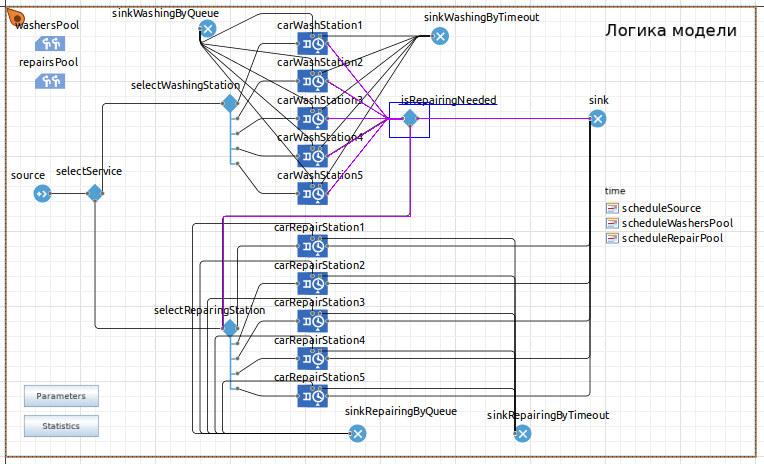
\includegraphics[scale=0.55]{carwashing_anylogic_model}
		\caption{Модель в среде \textit{AnyLogic}}
		\label{fig:carwashing_anylogic_model}
	\end{figure}
	
	Также была проанализирована загруженность данной модели. На данном графике видно процентное соотношение клиентов, которых упускает данное СТО на услуге мойки автомобилей. (Рисунок \ref{fig:carwashing_anylogic_washing})
	
	\begin{figure}[h]
		\centering 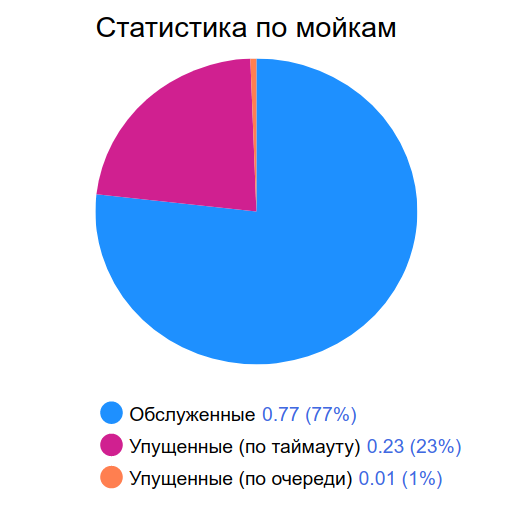
\includegraphics[scale=0.35]{carwashing_anylogic_washing}
		\caption{Диаграмма обслуженных клиентов на услуге мойки}
		\label{fig:carwashing_anylogic_washing}
	\end{figure}

	\newpage
	
	Можно видеть, что при достаточно серьёзном потоке клиентов СТО неплохо справляется с оказанием своих услуг и обрабатывает 77\% требований клиентов в среднем.\\
	
	На данном графике видно процентное соотношение клиентов, которых упускает данное СТО на услуге ремонта автомобилей. (Рисунок \ref{fig:carwashing_anylogic_repairing})
	
	\begin{figure}[h]
		\centering 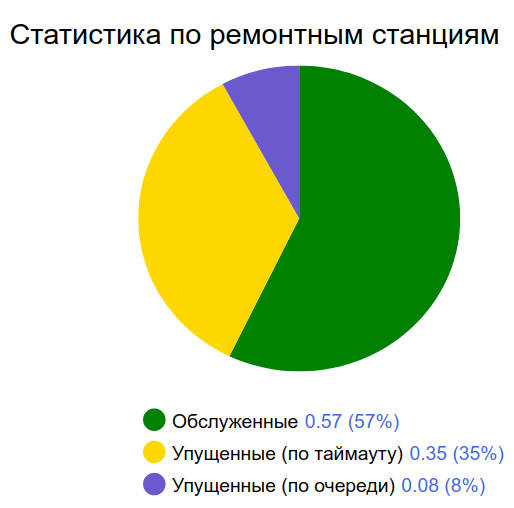
\includegraphics[scale=0.35]{carwashing_anylogic_repairing}
		\caption{Диаграмма обслуженных клиентов на услуге починки}
		\label{fig:carwashing_anylogic_repairing}
	\end{figure}
	
	Видно, что при достаточно серьёзном потоке клиентов СТО хуже справляется со своими обязанностями, но это может быть связано с фактором того, что много клиентов нуждается в достаточно трудоёмком сервисе.\\
	
	Также был построен график занятости сотрудников СТО. (Рисунок \ref{fig:carwashing_anylogic_workers})
	
	\begin{figure}[h]
		\centering 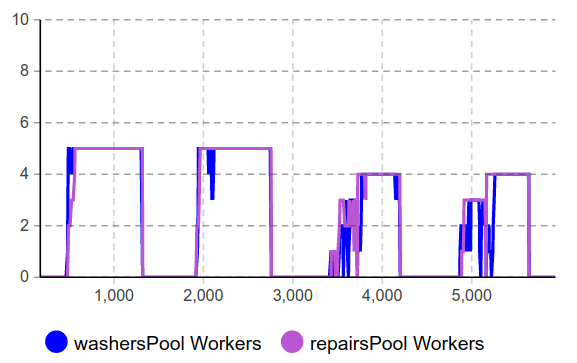
\includegraphics[scale=0.5]{carwashing_anylogic_workers}
		\caption{График занятости сотрудников СТО}
		\label{fig:carwashing_anylogic_workers}
	\end{figure}

	Можно видеть, что в выходные дни сотрудники полностью загруженны, а в рабочие дни бывают определённые скачки.
\end{document}
